\documentclass[1p]{elsarticle_modified}
%\bibliographystyle{elsarticle-num}

%\usepackage[colorlinks]{hyperref}
%\usepackage{abbrmath_seonhwa} %\Abb, \Ascr, \Acal ,\Abf, \Afrak
\usepackage{amsfonts}
\usepackage{amssymb}
\usepackage{amsmath}
\usepackage{amsthm}
\usepackage{scalefnt}
\usepackage{amsbsy}
\usepackage{kotex}
\usepackage{caption}
\usepackage{subfig}
\usepackage{color}
\usepackage{graphicx}
\usepackage{xcolor} %% white, black, red, green, blue, cyan, magenta, yellow
\usepackage{float}
\usepackage{setspace}
\usepackage{hyperref}

\usepackage{tikz}
\usetikzlibrary{arrows}

\usepackage{multirow}
\usepackage{array} % fixed length table
\usepackage{hhline}

%%%%%%%%%%%%%%%%%%%%%
\makeatletter
\renewcommand*\env@matrix[1][\arraystretch]{%
	\edef\arraystretch{#1}%
	\hskip -\arraycolsep
	\let\@ifnextchar\new@ifnextchar
	\array{*\c@MaxMatrixCols c}}
\makeatother %https://tex.stackexchange.com/questions/14071/how-can-i-increase-the-line-spacing-in-a-matrix
%%%%%%%%%%%%%%%

\usepackage[normalem]{ulem}

\newcommand{\msout}[1]{\ifmmode\text{\sout{\ensuremath{#1}}}\else\sout{#1}\fi}
%SOURCE: \msout is \stkout macro in https://tex.stackexchange.com/questions/20609/strikeout-in-math-mode

\newcommand{\cancel}[1]{
	\ifmmode
	{\color{red}\msout{#1}}
	\else
	{\color{red}\sout{#1}}
	\fi
}

\newcommand{\add}[1]{
	{\color{blue}\uwave{#1}}
}

\newcommand{\replace}[2]{
	\ifmmode
	{\color{red}\msout{#1}}{\color{blue}\uwave{#2}}
	\else
	{\color{red}\sout{#1}}{\color{blue}\uwave{#2}}
	\fi
}

\newcommand{\Sol}{\mathcal{S}} %segment
\newcommand{\D}{D} %diagram
\newcommand{\A}{\mathcal{A}} %arc


%%%%%%%%%%%%%%%%%%%%%%%%%%%%%5 test

\def\sl{\operatorname{\textup{SL}}(2,\Cbb)}
\def\psl{\operatorname{\textup{PSL}}(2,\Cbb)}
\def\quan{\mkern 1mu \triangleright \mkern 1mu}

\theoremstyle{definition}
\newtheorem{thm}{Theorem}[section]
\newtheorem{prop}[thm]{Proposition}
\newtheorem{lem}[thm]{Lemma}
\newtheorem{ques}[thm]{Question}
\newtheorem{cor}[thm]{Corollary}
\newtheorem{defn}[thm]{Definition}
\newtheorem{exam}[thm]{Example}
\newtheorem{rmk}[thm]{Remark}
\newtheorem{alg}[thm]{Algorithm}

\newcommand{\I}{\sqrt{-1}}
\begin{document}

%\begin{frontmatter}
%
%\title{Boundary parabolic representations of knots up to 8 crossings}
%
%%% Group authors per affiliation:
%\author{Yunhi Cho} 
%\address{Department of Mathematics, University of Seoul, Seoul, Korea}
%\ead{yhcho@uos.ac.kr}
%
%
%\author{Seonhwa Kim} %\fnref{s_kim}}
%\address{Center for Geometry and Physics, Institute for Basic Science, Pohang, 37673, Korea}
%\ead{ryeona17@ibs.re.kr}
%
%\author{Hyuk Kim}
%\address{Department of Mathematical Sciences, Seoul National University, Seoul 08826, Korea}
%\ead{hyukkim@snu.ac.kr}
%
%\author{Seokbeom Yoon}
%\address{Department of Mathematical Sciences, Seoul National University, Seoul, 08826,  Korea}
%\ead{sbyoon15@snu.ac.kr}
%
%\begin{abstract}
%We find all boundary parabolic representation of knots up to 8 crossings.
%
%\end{abstract}
%\begin{keyword}
%    \MSC[2010] 57M25 
%\end{keyword}
%
%\end{frontmatter}

%\linenumbers
%\tableofcontents
%
\newcommand\colored[1]{\textcolor{white}{\rule[-0.35ex]{0.8em}{1.4ex}}\kern-0.8em\color{red} #1}%
%\newcommand\colored[1]{\textcolor{white}{ #1}\kern-2.17ex	\textcolor{white}{ #1}\kern-1.81ex	\textcolor{white}{ #1}\kern-2.15ex\color{red}#1	}

{\Large $\underline{12n_{0016}~(K12n_{0016})}$}

\setlength{\tabcolsep}{10pt}
\renewcommand{\arraystretch}{1.6}
\vspace{1cm}\begin{tabular}{m{100pt}>{\centering\arraybackslash}m{274pt}}
\multirow{5}{120pt}{
	\centering
	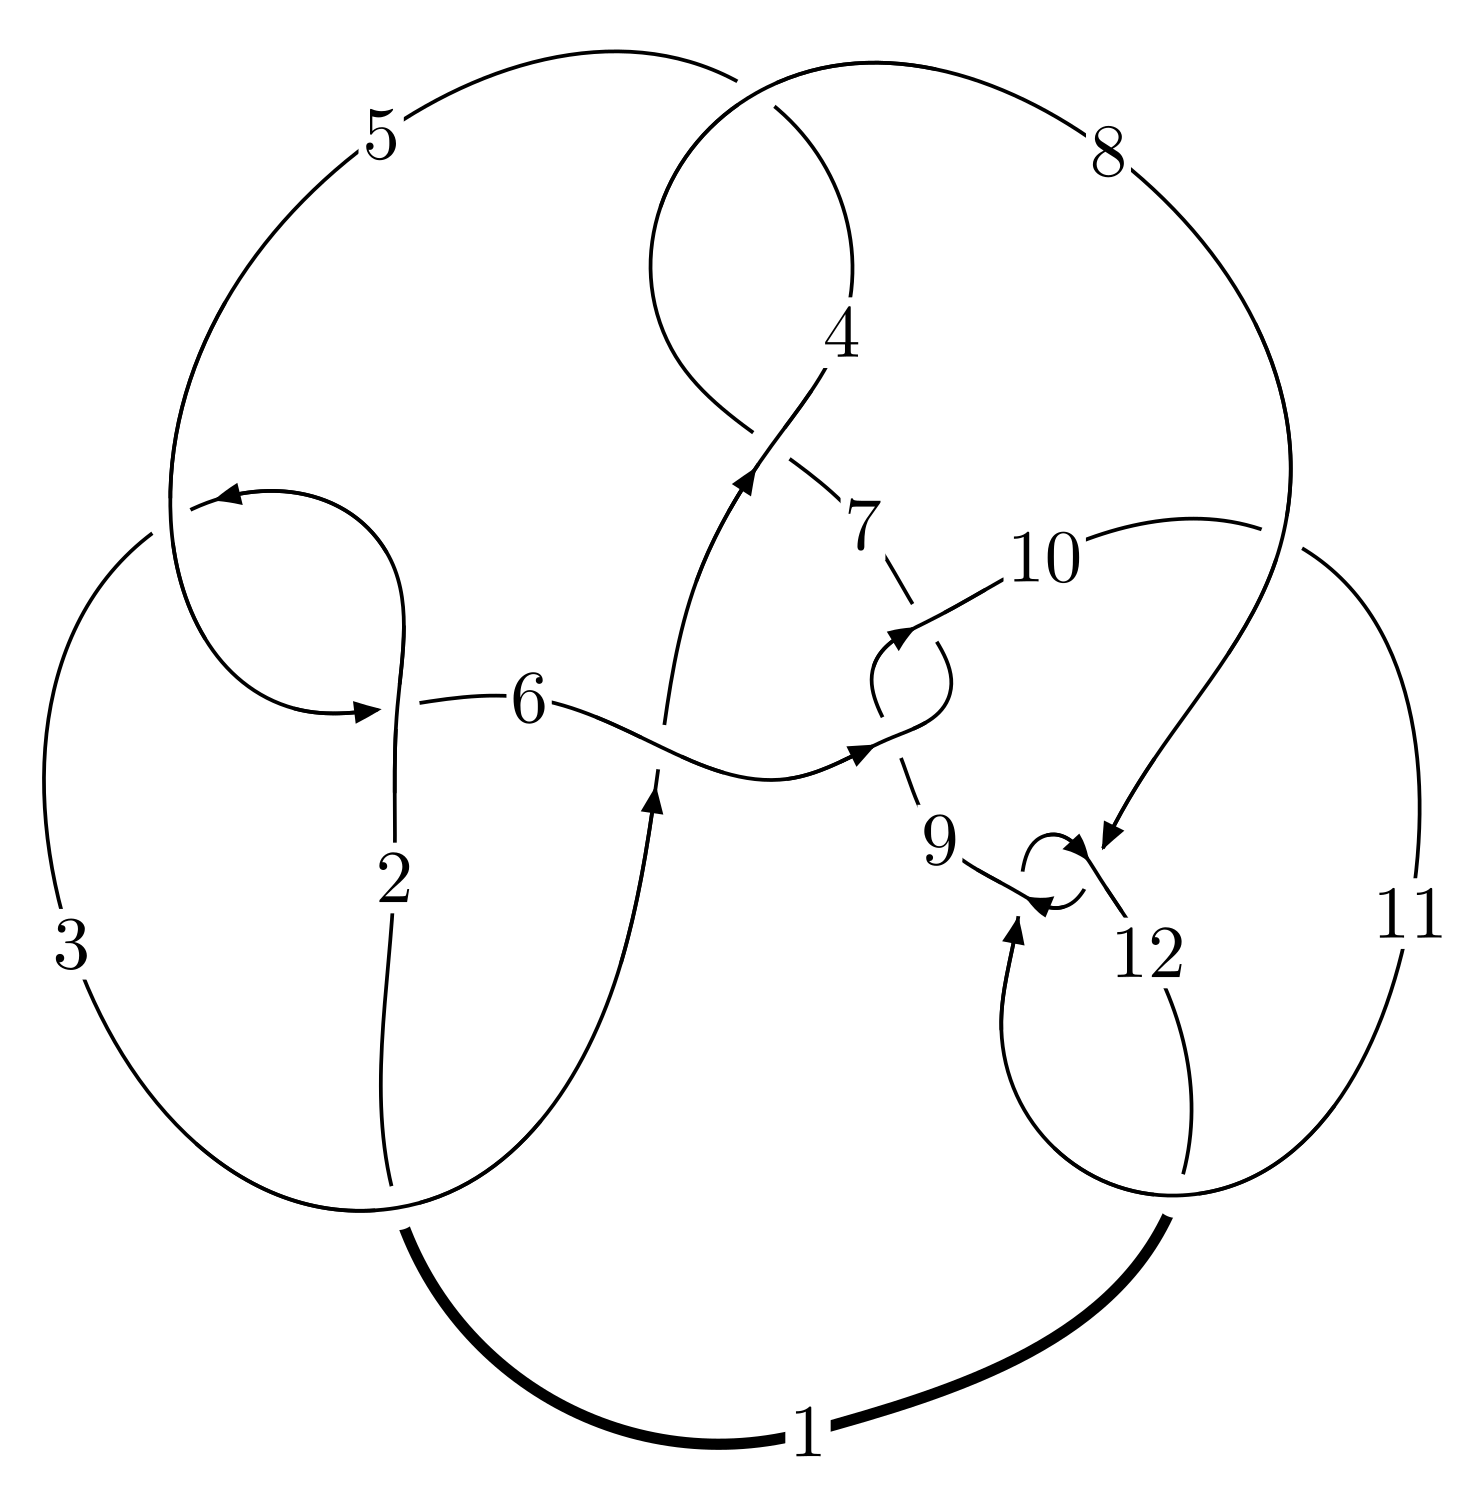
\includegraphics[width=112pt]{../../../GIT/diagram.site/Diagrams/png/2105_12n_0016.png}\\
\ \ \ A knot diagram\footnotemark}&
\allowdisplaybreaks
\textbf{Linearized knot diagam} \\
\cline{2-2}
 &
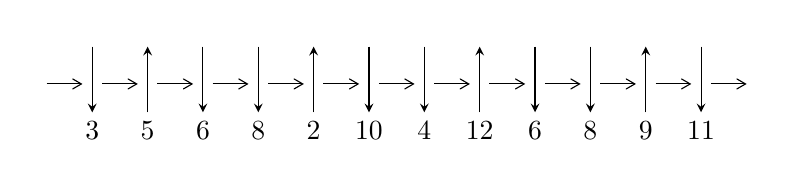
\begin{tikzpicture}[x=20pt, y=17pt]
	% nodes
	\node (C0) at (0, 0) {};
	\node (C1) at (1, 0) {};
	\node (C1U) at (1, +1) {};
	\node (C1D) at (1, -1) {3};

	\node (C2) at (2, 0) {};
	\node (C2U) at (2, +1) {};
	\node (C2D) at (2, -1) {5};

	\node (C3) at (3, 0) {};
	\node (C3U) at (3, +1) {};
	\node (C3D) at (3, -1) {6};

	\node (C4) at (4, 0) {};
	\node (C4U) at (4, +1) {};
	\node (C4D) at (4, -1) {8};

	\node (C5) at (5, 0) {};
	\node (C5U) at (5, +1) {};
	\node (C5D) at (5, -1) {2};

	\node (C6) at (6, 0) {};
	\node (C6U) at (6, +1) {};
	\node (C6D) at (6, -1) {10};

	\node (C7) at (7, 0) {};
	\node (C7U) at (7, +1) {};
	\node (C7D) at (7, -1) {4};

	\node (C8) at (8, 0) {};
	\node (C8U) at (8, +1) {};
	\node (C8D) at (8, -1) {12};

	\node (C9) at (9, 0) {};
	\node (C9U) at (9, +1) {};
	\node (C9D) at (9, -1) {6};

	\node (C10) at (10, 0) {};
	\node (C10U) at (10, +1) {};
	\node (C10D) at (10, -1) {8};

	\node (C11) at (11, 0) {};
	\node (C11U) at (11, +1) {};
	\node (C11D) at (11, -1) {9};

	\node (C12) at (12, 0) {};
	\node (C12U) at (12, +1) {};
	\node (C12D) at (12, -1) {11};
	\node (C13) at (13, 0) {};

	% arrows
	\draw[->,>={angle 60}]
	(C0) edge (C1) (C1) edge (C2) (C2) edge (C3) (C3) edge (C4) (C4) edge (C5) (C5) edge (C6) (C6) edge (C7) (C7) edge (C8) (C8) edge (C9) (C9) edge (C10) (C10) edge (C11) (C11) edge (C12) (C12) edge (C13) ;	\draw[->,>=stealth]
	(C1U) edge (C1D) (C2D) edge (C2U) (C3U) edge (C3D) (C4U) edge (C4D) (C5D) edge (C5U) (C6U) edge (C6D) (C7U) edge (C7D) (C8D) edge (C8U) (C9U) edge (C9D) (C10U) edge (C10D) (C11D) edge (C11U) (C12U) edge (C12D) ;
	\end{tikzpicture} \\
\hhline{~~} \\& 
\textbf{Solving Sequence} \\ \cline{2-2} 
 &
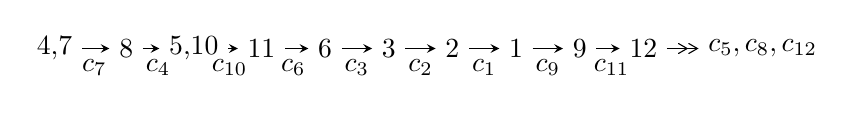
\begin{tikzpicture}[x=23pt, y=7pt]
	% node
	\node (A0) at (-1/8, 0) {4,7};
	\node (A1) at (1, 0) {8};
	\node (A2) at (33/16, 0) {5,10};
	\node (A3) at (25/8, 0) {11};
	\node (A4) at (33/8, 0) {6};
	\node (A5) at (41/8, 0) {3};
	\node (A6) at (49/8, 0) {2};
	\node (A7) at (57/8, 0) {1};
	\node (A8) at (65/8, 0) {9};
	\node (A9) at (73/8, 0) {12};
	\node (C1) at (1/2, -1) {$c_{7}$};
	\node (C2) at (3/2, -1) {$c_{4}$};
	\node (C3) at (21/8, -1) {$c_{10}$};
	\node (C4) at (29/8, -1) {$c_{6}$};
	\node (C5) at (37/8, -1) {$c_{3}$};
	\node (C6) at (45/8, -1) {$c_{2}$};
	\node (C7) at (53/8, -1) {$c_{1}$};
	\node (C8) at (61/8, -1) {$c_{9}$};
	\node (C9) at (69/8, -1) {$c_{11}$};
	\node (A10) at (11, 0) {$c_{5},c_{8},c_{12}$};

	% edge
	\draw[->,>=stealth]	
	(A0) edge (A1) (A1) edge (A2) (A2) edge (A3) (A3) edge (A4) (A4) edge (A5) (A5) edge (A6) (A6) edge (A7) (A7) edge (A8) (A8) edge (A9) ;
	\draw[->>,>={angle 60}]	
	(A9) edge (A10);
\end{tikzpicture} \\ 

\end{tabular} \\

\footnotetext{
The image of knot diagram is generated by the software ``\textbf{Draw programme}" developed by Andrew Bartholomew(\url{http://www.layer8.co.uk/maths/draw/index.htm\#Running-draw}), where we modified some parts for our purpose(\url{https://github.com/CATsTAILs/LinksPainter}).
}\phantom \\ \newline 
\centering \textbf{Ideals for irreducible components\footnotemark of $X_{\text{par}}$} 
 
\begin{align*}
I^u_{1}&=\langle 
b+u,\;224074 u^9+244456 u^8+\cdots+85463 a+346296,\\
\phantom{I^u_{1}}&\phantom{= \langle  }u^{10}+u^9-7 u^8-14 u^7+16 u^6+17 u^5-3 u^4-10 u^3-3 u^2+u-1\rangle \\
I^u_{2}&=\langle 
5.86389\times10^{37} u^{19}+1.09059\times10^{38} u^{18}+\cdots+1.52045\times10^{41} b-1.97465\times10^{40},\\
\phantom{I^u_{2}}&\phantom{= \langle  }-1.68947\times10^{39} u^{19}-3.22641\times10^{39} u^{18}+\cdots+1.21636\times10^{42} a-1.00257\times10^{42},\\
\phantom{I^u_{2}}&\phantom{= \langle  }u^{20}+2 u^{19}+\cdots-2048 u+1024\rangle \\
I^u_{3}&=\langle 
b,\;u^4 a-2 u^3 a-3 u^4- u^2 a+3 u^3+a^2+3 a u+7 u^2-5 u-4,\;u^5- u^4-2 u^3+u^2+u+1\rangle \\
\\
I^v_{1}&=\langle 
a,\;8286 v^9-14092 v^8+\cdots+8095 b+12581,\\
\phantom{I^v_{1}}&\phantom{= \langle  }v^{10}- v^9-2 v^8-19 v^7+12 v^6+35 v^5+50 v^4+34 v^3+17 v^2+5 v+1\rangle \\
\end{align*}
\raggedright * 4 irreducible components of $\dim_{\mathbb{C}}=0$, with total 50 representations.\\
\footnotetext{All coefficients of polynomials are rational numbers. But the coefficients are sometimes approximated in decimal forms when there is not enough margin.}
\newpage
\renewcommand{\arraystretch}{1}
\centering \section*{I. $I^u_{1}= \langle b+u,\;224074 u^9+244456 u^8+\cdots+85463 a+346296,\;u^{10}+u^9+\cdots+u-1 \rangle$}
\flushleft \textbf{(i) Arc colorings}\\
\begin{tabular}{m{7pt} m{180pt} m{7pt} m{180pt} }
\flushright $a_{4}=$&$\begin{pmatrix}0\\u\end{pmatrix}$ \\
\flushright $a_{7}=$&$\begin{pmatrix}1\\0\end{pmatrix}$ \\
\flushright $a_{8}=$&$\begin{pmatrix}1\\u^2\end{pmatrix}$ \\
\flushright $a_{5}=$&$\begin{pmatrix}- u\\- u^3+u\end{pmatrix}$ \\
\flushright $a_{10}=$&$\begin{pmatrix}-2.62188 u^{9}-2.86037 u^{8}+\cdots+12.1063 u-4.05200\\- u\end{pmatrix}$ \\
\flushright $a_{11}=$&$\begin{pmatrix}-2.43179 u^{9}-2.58767 u^{8}+\cdots+10.7229 u-4.29049\\0.0122626 u^{9}-0.0607046 u^{8}+\cdots-0.892515 u+0.0826088\end{pmatrix}$ \\
\flushright $a_{6}=$&$\begin{pmatrix}-0.238489 u^{9}-0.0483952 u^{8}+\cdots-1.43012 u-1.62188\\- u^2\end{pmatrix}$ \\
\flushright $a_{3}=$&$\begin{pmatrix}-0.367925 u^{9}-0.606110 u^{8}+\cdots+3.87427 u+0.559587\\-0.0122626 u^{9}+0.0607046 u^{8}+\cdots+0.892515 u-0.0826088\end{pmatrix}$ \\
\flushright $a_{2}=$&$\begin{pmatrix}-0.404257 u^{9}-0.758316 u^{8}+\cdots+4.08826 u+0.692697\\-0.122310 u^{9}-0.00902145 u^{8}+\cdots+0.758071 u-0.331594\end{pmatrix}$ \\
\flushright $a_{1}=$&$\begin{pmatrix}0.238489 u^{9}+0.0483952 u^{8}+\cdots+1.43012 u+1.62188\\-0.0826088 u^{9}-0.0948715 u^{8}+\cdots+0.428583 u-0.190094\end{pmatrix}$ \\
\flushright $a_{9}=$&$\begin{pmatrix}-2.81198 u^{9}-3.13308 u^{8}+\cdots+13.4897 u-3.81351\\u^3- u\end{pmatrix}$ \\
\flushright $a_{12}=$&$\begin{pmatrix}-1.14164 u^{9}-0.462949 u^{8}+\cdots-5.42663 u-7.69845\\0.122310 u^{9}+0.00902145 u^{8}+\cdots-0.758071 u+0.331594\end{pmatrix}$\\&\end{tabular}
\flushleft \textbf{(ii) Obstruction class $= -1$}\\~\\
\flushleft \textbf{(iii) Cusp Shapes $= -\frac{765256}{85463} u^9-\frac{1261184}{85463} u^8+\frac{4740376}{85463} u^7+\frac{14048256}{85463} u^6-\frac{4533392}{85463} u^5-\frac{19248384}{85463} u^4-\frac{7535280}{85463} u^3+\frac{7955648}{85463} u^2+\frac{7424384}{85463} u+\frac{490522}{85463}$}\\~\\
\newpage\renewcommand{\arraystretch}{1}
\flushleft \textbf{(iv) u-Polynomials at the component}\newline \\
\begin{tabular}{m{50pt}|m{274pt}}
Crossings & \hspace{64pt}u-Polynomials at each crossing \\
\hline $$\begin{aligned}c_{1},c_{12}\end{aligned}$$&$\begin{aligned}
&u^{10}+5 u^9+13 u^8+12 u^7-12 u^6-51 u^5-65 u^4-44 u^3-13 u^2+u+1
\end{aligned}$\\
\hline $$\begin{aligned}c_{2},c_{5},c_{8}\\c_{11}\end{aligned}$$&$\begin{aligned}
&u^{10}+3 u^9+7 u^8+10 u^7+12 u^6+13 u^5+11 u^4+10 u^3+5 u^2+3 u+1
\end{aligned}$\\
\hline $$\begin{aligned}c_{3},c_{10}\end{aligned}$$&$\begin{aligned}
&u^{10}-3 u^9-9 u^8+36 u^7-12 u^6-7 u^5-23 u^4+13 u^3+16 u^2+3 u+2
\end{aligned}$\\
\hline $$\begin{aligned}c_{4},c_{6},c_{7}\\c_{9}\end{aligned}$$&$\begin{aligned}
&u^{10}+u^9-7 u^8-14 u^7+16 u^6+17 u^5-3 u^4-10 u^3-3 u^2+u-1
\end{aligned}$\\
\hline
\end{tabular}\\~\\
\newpage\renewcommand{\arraystretch}{1}
\flushleft \textbf{(v) Riley Polynomials at the component}\newline \\
\begin{tabular}{m{50pt}|m{274pt}}
Crossings & \hspace{64pt}Riley Polynomials at each crossing \\
\hline $$\begin{aligned}c_{1},c_{12}\end{aligned}$$&$\begin{aligned}
&y^{10}+y^9+\cdots-27 y+1
\end{aligned}$\\
\hline $$\begin{aligned}c_{2},c_{5},c_{8}\\c_{11}\end{aligned}$$&$\begin{aligned}
&y^{10}+5 y^9+13 y^8+12 y^7-12 y^6-51 y^5-65 y^4-44 y^3-13 y^2+y+1
\end{aligned}$\\
\hline $$\begin{aligned}c_{3},c_{10}\end{aligned}$$&$\begin{aligned}
&y^{10}-27 y^9+\cdots+55 y+4
\end{aligned}$\\
\hline $$\begin{aligned}c_{4},c_{6},c_{7}\\c_{9}\end{aligned}$$&$\begin{aligned}
&y^{10}-15 y^9+\cdots+5 y+1
\end{aligned}$\\
\hline
\end{tabular}\\~\\
\newpage\flushleft \textbf{(vi) Complex Volumes and Cusp Shapes}
$$\begin{array}{c|c|c}  
\text{Solutions to }I^u_{1}& \I (\text{vol} + \sqrt{-1}CS) & \text{Cusp shape}\\
 \hline 
\begin{aligned}
u &= \phantom{-}1.051110 + 0.169733 I \\
a &= \phantom{-}0.075124 + 0.218323 I \\
b &= -1.051110 - 0.169733 I\end{aligned}
 & -6.66754 - 7.26680 I & -14.1481 + 8.5135 I \\ \hline\begin{aligned}
u &= \phantom{-}1.051110 - 0.169733 I \\
a &= \phantom{-}0.075124 - 0.218323 I \\
b &= -1.051110 + 0.169733 I\end{aligned}
 & -6.66754 + 7.26680 I & -14.1481 - 8.5135 I \\ \hline\begin{aligned}
u &= -0.766019\phantom{ +0.000000I} \\
a &= \phantom{-}0.342395\phantom{ +0.000000I} \\
b &= \phantom{-}0.766019\phantom{ +0.000000I}\end{aligned}
 & -1.35955\phantom{ +0.000000I} & -6.41950\phantom{ +0.000000I} \\ \hline\begin{aligned}
u &= -0.505971 + 0.548673 I \\
a &= \phantom{-}0.308348 + 0.874136 I \\
b &= \phantom{-}0.505971 - 0.548673 I\end{aligned}
 & -1.23733 + 1.36545 I & -9.59143 - 3.61875 I \\ \hline\begin{aligned}
u &= -0.505971 - 0.548673 I \\
a &= \phantom{-}0.308348 - 0.874136 I \\
b &= \phantom{-}0.505971 + 0.548673 I\end{aligned}
 & -1.23733 - 1.36545 I & -9.59143 + 3.61875 I \\ \hline\begin{aligned}
u &= \phantom{-}0.171353 + 0.321669 I \\
a &= -4.31436 + 8.42917 I \\
b &= -0.171353 - 0.321669 I\end{aligned}
 & -0.16069 - 3.80568 I & \phantom{-}19.6494 + 42.7056 I \\ \hline\begin{aligned}
u &= \phantom{-}0.171353 - 0.321669 I \\
a &= -4.31436 - 8.42917 I \\
b &= -0.171353 + 0.321669 I\end{aligned}
 & -0.16069 + 3.80568 I & \phantom{-}19.6494 - 42.7056 I \\ \hline\begin{aligned}
u &= -2.11995 + 1.24678 I \\
a &= \phantom{-}0.704601 + 0.550226 I \\
b &= \phantom{-}2.11995 - 1.24678 I\end{aligned}
 & \phantom{-}17.3702 + 13.6949 I & -8.24581 - 5.79353 I \\ \hline\begin{aligned}
u &= -2.11995 - 1.24678 I \\
a &= \phantom{-}0.704601 - 0.550226 I \\
b &= \phantom{-}2.11995 + 1.24678 I\end{aligned}
 & \phantom{-}17.3702 - 13.6949 I & -8.24581 + 5.79353 I \\ \hline\begin{aligned}
u &= \phantom{-}2.57293\phantom{ +0.000000I} \\
a &= -0.889824\phantom{ +0.000000I} \\
b &= -2.57293\phantom{ +0.000000I}\end{aligned}
 & -13.9598\phantom{ +0.000000I} & -4.90870\phantom{ +0.000000I}\\
 \hline 
 \end{array}$$\newpage\newpage\renewcommand{\arraystretch}{1}
\centering \section*{II. $I^u_{2}= \langle 5.86\times10^{37} u^{19}+1.09\times10^{38} u^{18}+\cdots+1.52\times10^{41} b-1.97\times10^{40},\;-1.69\times10^{39} u^{19}-3.23\times10^{39} u^{18}+\cdots+1.22\times10^{42} a-1.00\times10^{42},\;u^{20}+2 u^{19}+\cdots-2048 u+1024 \rangle$}
\flushleft \textbf{(i) Arc colorings}\\
\begin{tabular}{m{7pt} m{180pt} m{7pt} m{180pt} }
\flushright $a_{4}=$&$\begin{pmatrix}0\\u\end{pmatrix}$ \\
\flushright $a_{7}=$&$\begin{pmatrix}1\\0\end{pmatrix}$ \\
\flushright $a_{8}=$&$\begin{pmatrix}1\\u^2\end{pmatrix}$ \\
\flushright $a_{5}=$&$\begin{pmatrix}- u\\- u^3+u\end{pmatrix}$ \\
\flushright $a_{10}=$&$\begin{pmatrix}0.00138896 u^{19}+0.00265251 u^{18}+\cdots+3.64638 u+0.824235\\-0.000385667 u^{19}-0.000717282 u^{18}+\cdots-1.18247 u+0.129872\end{pmatrix}$ \\
\flushright $a_{11}=$&$\begin{pmatrix}0.00151255 u^{19}+0.00313681 u^{18}+\cdots+3.14973 u+0.822778\\-0.000451559 u^{19}-0.000899794 u^{18}+\cdots-0.823414 u-0.112935\end{pmatrix}$ \\
\flushright $a_{6}=$&$\begin{pmatrix}0.000295502 u^{19}+0.000835151 u^{18}+\cdots-2.41530 u+0.836394\\-1.74761\times10^{-6} u^{19}-0.0000459509 u^{18}+\cdots+0.619191 u+0.0512561\end{pmatrix}$ \\
\flushright $a_{3}=$&$\begin{pmatrix}-0.000175793 u^{19}-0.000736748 u^{18}+\cdots+3.47292 u-1.24551\\0.000101127 u^{19}+0.000225173 u^{18}+\cdots+0.697375 u+0.189635\end{pmatrix}$ \\
\flushright $a_{2}=$&$\begin{pmatrix}-0.000515937 u^{19}-0.00143281 u^{18}+\cdots+3.99150 u-1.66721\\0.000576429 u^{19}+0.00110414 u^{18}+\cdots+0.494790 u+0.627482\end{pmatrix}$ \\
\flushright $a_{1}=$&$\begin{pmatrix}-0.000293754 u^{19}-0.000789200 u^{18}+\cdots+1.79611 u-0.887650\\0.000158683 u^{19}+0.000288930 u^{18}+\cdots+0.506931 u+0.257788\end{pmatrix}$ \\
\flushright $a_{9}=$&$\begin{pmatrix}0.00144125 u^{19}+0.00289745 u^{18}+\cdots+2.51554 u+1.04162\\-0.000525250 u^{19}-0.000988354 u^{18}+\cdots-1.00784 u+0.125174\end{pmatrix}$ \\
\flushright $a_{12}=$&$\begin{pmatrix}0.000756916 u^{19}+0.00212323 u^{18}+\cdots-1.07571 u+3.13147\\-0.000291771 u^{19}-0.000735805 u^{18}+\cdots-0.338968 u-0.810783\end{pmatrix}$\\&\end{tabular}
\flushleft \textbf{(ii) Obstruction class $= -1$}\\~\\
\flushleft \textbf{(iii) Cusp Shapes $= -0.00176167 u^{19}-0.00309564 u^{18}+\cdots-12.6991 u-1.09946$}\\~\\
\newpage\renewcommand{\arraystretch}{1}
\flushleft \textbf{(iv) u-Polynomials at the component}\newline \\
\begin{tabular}{m{50pt}|m{274pt}}
Crossings & \hspace{64pt}u-Polynomials at each crossing \\
\hline $$\begin{aligned}c_{1},c_{12}\end{aligned}$$&$\begin{aligned}
&u^{20}+19 u^{19}+\cdots+175 u+1
\end{aligned}$\\
\hline $$\begin{aligned}c_{2},c_{5},c_{8}\\c_{11}\end{aligned}$$&$\begin{aligned}
&u^{20}+5 u^{19}+\cdots+5 u+1
\end{aligned}$\\
\hline $$\begin{aligned}c_{3},c_{10}\end{aligned}$$&$\begin{aligned}
&u^{20}-5 u^{19}+\cdots+2619 u+641
\end{aligned}$\\
\hline $$\begin{aligned}c_{4},c_{6},c_{7}\\c_{9}\end{aligned}$$&$\begin{aligned}
&u^{20}+2 u^{19}+\cdots-2048 u+1024
\end{aligned}$\\
\hline
\end{tabular}\\~\\
\newpage\renewcommand{\arraystretch}{1}
\flushleft \textbf{(v) Riley Polynomials at the component}\newline \\
\begin{tabular}{m{50pt}|m{274pt}}
Crossings & \hspace{64pt}Riley Polynomials at each crossing \\
\hline $$\begin{aligned}c_{1},c_{12}\end{aligned}$$&$\begin{aligned}
&y^{20}-29 y^{19}+\cdots-13889 y+1
\end{aligned}$\\
\hline $$\begin{aligned}c_{2},c_{5},c_{8}\\c_{11}\end{aligned}$$&$\begin{aligned}
&y^{20}+19 y^{19}+\cdots+175 y+1
\end{aligned}$\\
\hline $$\begin{aligned}c_{3},c_{10}\end{aligned}$$&$\begin{aligned}
&y^{20}-53 y^{19}+\cdots+71819743 y+410881
\end{aligned}$\\
\hline $$\begin{aligned}c_{4},c_{6},c_{7}\\c_{9}\end{aligned}$$&$\begin{aligned}
&y^{20}-50 y^{19}+\cdots+4194304 y+1048576
\end{aligned}$\\
\hline
\end{tabular}\\~\\
\newpage\flushleft \textbf{(vi) Complex Volumes and Cusp Shapes}
$$\begin{array}{c|c|c}  
\text{Solutions to }I^u_{2}& \I (\text{vol} + \sqrt{-1}CS) & \text{Cusp shape}\\
 \hline 
\begin{aligned}
u &= -0.804594 + 0.696559 I \\
a &= -0.002315 - 0.280709 I \\
b &= -1.396170 - 0.196408 I\end{aligned}
 & -4.73849 + 3.00338 I & -7.64371 - 3.35763 I \\ \hline\begin{aligned}
u &= -0.804594 - 0.696559 I \\
a &= -0.002315 + 0.280709 I \\
b &= -1.396170 + 0.196408 I\end{aligned}
 & -4.73849 - 3.00338 I & -7.64371 + 3.35763 I \\ \hline\begin{aligned}
u &= -0.257283 + 0.651285 I \\
a &= -1.12449 - 2.84653 I \\
b &= \phantom{-}0.257283 + 0.651285 I\end{aligned}
 & -0.537213\phantom{ +0.000000I} &                  -6
-1.350198 + 0. 10   I\phantom{ +0.000000I} \\ \hline\begin{aligned}
u &= -0.257283 - 0.651285 I \\
a &= -1.12449 + 2.84653 I \\
b &= \phantom{-}0.257283 - 0.651285 I\end{aligned}
 & -0.537213\phantom{ +0.000000I} &                  -6
-1.350198 + 0. 10   I\phantom{ +0.000000I} \\ \hline\begin{aligned}
u &= \phantom{-}1.396170 + 0.196408 I \\
a &= \phantom{-}0.160795 + 0.137994 I \\
b &= \phantom{-}0.804594 - 0.696559 I\end{aligned}
 & -4.73849 + 3.00338 I & -7.64371 - 3.35763 I \\ \hline\begin{aligned}
u &= \phantom{-}1.396170 - 0.196408 I \\
a &= \phantom{-}0.160795 - 0.137994 I \\
b &= \phantom{-}0.804594 + 0.696559 I\end{aligned}
 & -4.73849 - 3.00338 I & -7.64371 + 3.35763 I \\ \hline\begin{aligned}
u &= -0.204722 + 0.532348 I \\
a &= \phantom{-}1.241470 + 0.214157 I \\
b &= -0.241836 - 0.217250 I\end{aligned}
 & -0.35106 + 1.66079 I & -2.53678 - 3.96410 I \\ \hline\begin{aligned}
u &= -0.204722 - 0.532348 I \\
a &= \phantom{-}1.241470 - 0.214157 I \\
b &= -0.241836 + 0.217250 I\end{aligned}
 & -0.35106 - 1.66079 I & -2.53678 + 3.96410 I \\ \hline\begin{aligned}
u &= \phantom{-}0.241836 + 0.217250 I \\
a &= \phantom{-}0.42599 + 2.16885 I \\
b &= \phantom{-}0.204722 - 0.532348 I\end{aligned}
 & -0.35106 + 1.66079 I & -2.53678 - 3.96410 I \\ \hline\begin{aligned}
u &= \phantom{-}0.241836 - 0.217250 I \\
a &= \phantom{-}0.42599 - 2.16885 I \\
b &= \phantom{-}0.204722 + 0.532348 I\end{aligned}
 & -0.35106 - 1.66079 I & -2.53678 + 3.96410 I\\
 \hline 
 \end{array}$$\newpage$$\begin{array}{c|c|c}  
\text{Solutions to }I^u_{2}& \I (\text{vol} + \sqrt{-1}CS) & \text{Cusp shape}\\
 \hline 
\begin{aligned}
u &= -0.55408 + 2.01462 I \\
a &= -0.191665 - 0.696885 I \\
b &= \phantom{-}0.55408 + 2.01462 I\end{aligned}
 & -4.58401\phantom{ +0.000000I} & -9.53898 + 0. I\phantom{ +0.000000I} \\ \hline\begin{aligned}
u &= -0.55408 - 2.01462 I \\
a &= -0.191665 + 0.696885 I \\
b &= \phantom{-}0.55408 - 2.01462 I\end{aligned}
 & -4.58401\phantom{ +0.000000I} & -9.53898 + 0. I\phantom{ +0.000000I} \\ \hline\begin{aligned}
u &= \phantom{-}2.55394 + 0.67960 I \\
a &= \phantom{-}0.797707 - 0.266076 I \\
b &= \phantom{-}2.56756 + 0.95364 I\end{aligned}
 & -18.4617 - 6.7670 I & -6.82707 + 2.49268 I \\ \hline\begin{aligned}
u &= \phantom{-}2.55394 - 0.67960 I \\
a &= \phantom{-}0.797707 + 0.266076 I \\
b &= \phantom{-}2.56756 - 0.95364 I\end{aligned}
 & -18.4617 + 6.7670 I & -6.82707 - 2.49268 I \\ \hline\begin{aligned}
u &= -2.56756 + 0.95364 I \\
a &= -0.741704 - 0.329004 I \\
b &= -2.55394 + 0.67960 I\end{aligned}
 & -18.4617 + 6.7670 I & -6.82707 - 2.49268 I \\ \hline\begin{aligned}
u &= -2.56756 - 0.95364 I \\
a &= -0.741704 + 0.329004 I \\
b &= -2.55394 - 0.67960 I\end{aligned}
 & -18.4617 - 6.7670 I & -6.82707 + 2.49268 I \\ \hline\begin{aligned}
u &= \phantom{-}2.62678 + 1.73277 I \\
a &= -0.171297 + 0.112997 I \\
b &= -2.62678 + 1.73277 I\end{aligned}
 & -12.4152\phantom{ +0.000000I} & -9.95005 + 0. I\phantom{ +0.000000I} \\ \hline\begin{aligned}
u &= \phantom{-}2.62678 - 1.73277 I \\
a &= -0.171297 - 0.112997 I \\
b &= -2.62678 - 1.73277 I\end{aligned}
 & -12.4152\phantom{ +0.000000I} & -9.95005 + 0. I\phantom{ +0.000000I} \\ \hline\begin{aligned}
u &= -3.43049 + 0.37740 I \\
a &= \phantom{-}0.605506 + 0.066614 I \\
b &= \phantom{-}3.43049 + 0.37740 I\end{aligned}
 & \phantom{-}15.2909\phantom{ +0.000000I} & -9.14565 + 0. I\phantom{ +0.000000I} \\ \hline\begin{aligned}
u &= -3.43049 - 0.37740 I \\
a &= \phantom{-}0.605506 - 0.066614 I \\
b &= \phantom{-}3.43049 - 0.37740 I\end{aligned}
 & \phantom{-}15.2909\phantom{ +0.000000I} & -9.14565 + 0. I\phantom{ +0.000000I}\\
 \hline 
 \end{array}$$\newpage\newpage\renewcommand{\arraystretch}{1}
\centering \section*{III. $I^u_{3}= \langle b,\;u^4 a-3 u^4+\cdots+a^2-4,\;u^5- u^4-2 u^3+u^2+u+1 \rangle$}
\flushleft \textbf{(i) Arc colorings}\\
\begin{tabular}{m{7pt} m{180pt} m{7pt} m{180pt} }
\flushright $a_{4}=$&$\begin{pmatrix}0\\u\end{pmatrix}$ \\
\flushright $a_{7}=$&$\begin{pmatrix}1\\0\end{pmatrix}$ \\
\flushright $a_{8}=$&$\begin{pmatrix}1\\u^2\end{pmatrix}$ \\
\flushright $a_{5}=$&$\begin{pmatrix}- u\\- u^3+u\end{pmatrix}$ \\
\flushright $a_{10}=$&$\begin{pmatrix}a\\0\end{pmatrix}$ \\
\flushright $a_{11}=$&$\begin{pmatrix}u^2 a+a\\u^4 a\end{pmatrix}$ \\
\flushright $a_{6}=$&$\begin{pmatrix}1\\0\end{pmatrix}$ \\
\flushright $a_{3}=$&$\begin{pmatrix}u\\u\end{pmatrix}$ \\
\flushright $a_{2}=$&$\begin{pmatrix}u^4- u^2-1\\u^4-2 u^2\end{pmatrix}$ \\
\flushright $a_{1}=$&$\begin{pmatrix}-1\\- u^2\end{pmatrix}$ \\
\flushright $a_{9}=$&$\begin{pmatrix}a\\0\end{pmatrix}$ \\
\flushright $a_{12}=$&$\begin{pmatrix}u^4+u^2 a-2 u^3- u^2+a+3 u\\u^4 a\end{pmatrix}$\\&\end{tabular}
\flushleft \textbf{(ii) Obstruction class $= 1$}\\~\\
\flushleft \textbf{(iii) Cusp Shapes $= 2 u^4 a+3 u^3 a+3 u^4-5 u^2 a+u^3-5 a u-7 u^2- a-3 u-6$}\\~\\
\newpage\renewcommand{\arraystretch}{1}
\flushleft \textbf{(iv) u-Polynomials at the component}\newline \\
\begin{tabular}{m{50pt}|m{274pt}}
Crossings & \hspace{64pt}u-Polynomials at each crossing \\
\hline $$\begin{aligned}c_{1}\end{aligned}$$&$\begin{aligned}
&(u^5-3 u^4+4 u^3- u^2- u+1)^2
\end{aligned}$\\
\hline $$\begin{aligned}c_{2}\end{aligned}$$&$\begin{aligned}
&(u^5- u^4+2 u^3- u^2+u-1)^2
\end{aligned}$\\
\hline $$\begin{aligned}c_{3},c_{4}\end{aligned}$$&$\begin{aligned}
&(u^5+u^4-2 u^3- u^2+u-1)^2
\end{aligned}$\\
\hline $$\begin{aligned}c_{5}\end{aligned}$$&$\begin{aligned}
&(u^5+u^4+2 u^3+u^2+u+1)^2
\end{aligned}$\\
\hline $$\begin{aligned}c_{6},c_{9}\end{aligned}$$&$\begin{aligned}
&u^{10}
\end{aligned}$\\
\hline $$\begin{aligned}c_{7}\end{aligned}$$&$\begin{aligned}
&(u^5- u^4-2 u^3+u^2+u+1)^2
\end{aligned}$\\
\hline $$\begin{aligned}c_{8},c_{10},c_{12}\end{aligned}$$&$\begin{aligned}
&(u^2+u+1)^5
\end{aligned}$\\
\hline $$\begin{aligned}c_{11}\end{aligned}$$&$\begin{aligned}
&(u^2- u+1)^5
\end{aligned}$\\
\hline
\end{tabular}\\~\\
\newpage\renewcommand{\arraystretch}{1}
\flushleft \textbf{(v) Riley Polynomials at the component}\newline \\
\begin{tabular}{m{50pt}|m{274pt}}
Crossings & \hspace{64pt}Riley Polynomials at each crossing \\
\hline $$\begin{aligned}c_{1}\end{aligned}$$&$\begin{aligned}
&(y^5- y^4+8 y^3-3 y^2+3 y-1)^2
\end{aligned}$\\
\hline $$\begin{aligned}c_{2},c_{5}\end{aligned}$$&$\begin{aligned}
&(y^5+3 y^4+4 y^3+y^2- y-1)^2
\end{aligned}$\\
\hline $$\begin{aligned}c_{3},c_{4},c_{7}\end{aligned}$$&$\begin{aligned}
&(y^5-5 y^4+8 y^3-3 y^2- y-1)^2
\end{aligned}$\\
\hline $$\begin{aligned}c_{6},c_{9}\end{aligned}$$&$\begin{aligned}
&y^{10}
\end{aligned}$\\
\hline $$\begin{aligned}c_{8},c_{10},c_{11}\\c_{12}\end{aligned}$$&$\begin{aligned}
&(y^2+y+1)^5
\end{aligned}$\\
\hline
\end{tabular}\\~\\
\newpage\flushleft \textbf{(vi) Complex Volumes and Cusp Shapes}
$$\begin{array}{c|c|c}  
\text{Solutions to }I^u_{3}& \I (\text{vol} + \sqrt{-1}CS) & \text{Cusp shape}\\
 \hline 
\begin{aligned}
u &= -1.21774\phantom{ +0.000000I} \\
a &= -0.337181 + 0.584015 I \\
b &= \phantom{-0.000000 } 0\end{aligned}
 & -2.40108 + 2.02988 I & -6.80799 - 1.95361 I \\ \hline\begin{aligned}
u &= -1.21774\phantom{ +0.000000I} \\
a &= -0.337181 - 0.584015 I \\
b &= \phantom{-0.000000 } 0\end{aligned}
 & -2.40108 - 2.02988 I & -6.80799 + 1.95361 I \\ \hline\begin{aligned}
u &= -0.309916 + 0.549911 I \\
a &= \phantom{-}2.50919 + 0.05217 I \\
b &= \phantom{-0.000000 } 0\end{aligned}
 & -0.32910 + 3.56046 I & -7.97351 - 2.70956 I \\ \hline\begin{aligned}
u &= -0.309916 + 0.549911 I \\
a &= -1.20942 - 2.19910 I \\
b &= \phantom{-0.000000 } 0\end{aligned}
 & -0.329100 - 0.499304 I & \phantom{-}1.93681 - 0.71136 I \\ \hline\begin{aligned}
u &= -0.309916 - 0.549911 I \\
a &= \phantom{-}2.50919 - 0.05217 I \\
b &= \phantom{-0.000000 } 0\end{aligned}
 & -0.32910 - 3.56046 I & -7.97351 + 2.70956 I \\ \hline\begin{aligned}
u &= -0.309916 - 0.549911 I \\
a &= -1.20942 + 2.19910 I \\
b &= \phantom{-0.000000 } 0\end{aligned}
 & -0.329100 + 0.499304 I & \phantom{-}1.93681 + 0.71136 I \\ \hline\begin{aligned}
u &= \phantom{-}1.41878 + 0.21917 I \\
a &= -0.358089 - 0.327409 I \\
b &= \phantom{-0.000000 } 0\end{aligned}
 & -5.87256 - 6.43072 I & -8.34383 + 2.96651 I \\ \hline\begin{aligned}
u &= \phantom{-}1.41878 + 0.21917 I \\
a &= -0.104500 + 0.473819 I \\
b &= \phantom{-0.000000 } 0\end{aligned}
 & -5.87256 - 2.37095 I & -12.81148 + 1.72217 I \\ \hline\begin{aligned}
u &= \phantom{-}1.41878 - 0.21917 I \\
a &= -0.358089 + 0.327409 I \\
b &= \phantom{-0.000000 } 0\end{aligned}
 & -5.87256 + 6.43072 I & -8.34383 - 2.96651 I \\ \hline\begin{aligned}
u &= \phantom{-}1.41878 - 0.21917 I \\
a &= -0.104500 - 0.473819 I \\
b &= \phantom{-0.000000 } 0\end{aligned}
 & -5.87256 + 2.37095 I & -12.81148 - 1.72217 I\\
 \hline 
 \end{array}$$\newpage\newpage\renewcommand{\arraystretch}{1}
\centering \section*{IV. $I^v_{1}= \langle a,\;8286 v^9-14092 v^8+\cdots+8095 b+12581,\;v^{10}- v^9+\cdots+5 v+1 \rangle$}
\flushleft \textbf{(i) Arc colorings}\\
\begin{tabular}{m{7pt} m{180pt} m{7pt} m{180pt} }
\flushright $a_{4}=$&$\begin{pmatrix}v\\0\end{pmatrix}$ \\
\flushright $a_{7}=$&$\begin{pmatrix}1\\0\end{pmatrix}$ \\
\flushright $a_{8}=$&$\begin{pmatrix}1\\0\end{pmatrix}$ \\
\flushright $a_{5}=$&$\begin{pmatrix}v\\0\end{pmatrix}$ \\
\flushright $a_{10}=$&$\begin{pmatrix}0\\-1.02359 v^{9}+1.74083 v^{8}+\cdots-2.14256 v-1.55417\end{pmatrix}$ \\
\flushright $a_{11}=$&$\begin{pmatrix}1.02359 v^{9}-1.74083 v^{8}+\cdots+2.14256 v+1.55417\\-1.02359 v^{9}+1.74083 v^{8}+\cdots-2.14256 v-1.55417\end{pmatrix}$ \\
\flushright $a_{6}=$&$\begin{pmatrix}1\\0.566770 v^{9}-0.910562 v^{8}+\cdots+1.12069 v-2.46844\end{pmatrix}$ \\
\flushright $a_{3}=$&$\begin{pmatrix}0.343792 v^{9}-0.433107 v^{8}+\cdots+6.30229 v+0.566770\\-1.56677 v^{9}+1.91056 v^{8}+\cdots-18.1207 v-2.53156\end{pmatrix}$ \\
\flushright $a_{2}=$&$\begin{pmatrix}0.433107 v^{9}-0.556763 v^{8}+\cdots+6.45448 v+0.910562\\-1.56677 v^{9}+1.91056 v^{8}+\cdots-18.1207 v-2.53156\end{pmatrix}$ \\
\flushright $a_{1}=$&$\begin{pmatrix}-1\\-0.566770 v^{9}+0.910562 v^{8}+\cdots-1.12069 v+2.46844\end{pmatrix}$ \\
\flushright $a_{9}=$&$\begin{pmatrix}-1.02359 v^{9}+1.74083 v^{8}+\cdots-2.14256 v-1.55417\\-0.515256 v^{9}+0.785300 v^{8}+\cdots-0.966523 v+2.10241\end{pmatrix}$ \\
\flushright $a_{12}=$&$\begin{pmatrix}-1.96479 v^{9}+3.18777 v^{8}+\cdots-3.92341 v+1.99444\\1.39802 v^{9}-2.27721 v^{8}+\cdots+2.80272 v-0.526004\end{pmatrix}$\\&\end{tabular}
\flushleft \textbf{(ii) Obstruction class $= 1$}\\~\\
\flushleft \textbf{(iii) Cusp Shapes $= -\frac{4097}{1619} v^9+\frac{9450}{1619} v^8+\frac{1665}{1619} v^7+\frac{67341}{1619} v^6-\frac{147227}{1619} v^5-\frac{55323}{1619} v^4-\frac{14483}{1619} v^3+\frac{69031}{1619} v^2+\frac{28097}{1619} v-\frac{3358}{1619}$}\\~\\
\newpage\renewcommand{\arraystretch}{1}
\flushleft \textbf{(iv) u-Polynomials at the component}\newline \\
\begin{tabular}{m{50pt}|m{274pt}}
Crossings & \hspace{64pt}u-Polynomials at each crossing \\
\hline $$\begin{aligned}c_{1},c_{3},c_{5}\end{aligned}$$&$\begin{aligned}
&(u^2- u+1)^5
\end{aligned}$\\
\hline $$\begin{aligned}c_{2}\end{aligned}$$&$\begin{aligned}
&(u^2+u+1)^5
\end{aligned}$\\
\hline $$\begin{aligned}c_{4},c_{7}\end{aligned}$$&$\begin{aligned}
&u^{10}
\end{aligned}$\\
\hline $$\begin{aligned}c_{6}\end{aligned}$$&$\begin{aligned}
&(u^5+u^4-2 u^3- u^2+u-1)^2
\end{aligned}$\\
\hline $$\begin{aligned}c_{8}\end{aligned}$$&$\begin{aligned}
&(u^5- u^4+2 u^3- u^2+u-1)^2
\end{aligned}$\\
\hline $$\begin{aligned}c_{9},c_{10}\end{aligned}$$&$\begin{aligned}
&(u^5- u^4-2 u^3+u^2+u+1)^2
\end{aligned}$\\
\hline $$\begin{aligned}c_{11}\end{aligned}$$&$\begin{aligned}
&(u^5+u^4+2 u^3+u^2+u+1)^2
\end{aligned}$\\
\hline $$\begin{aligned}c_{12}\end{aligned}$$&$\begin{aligned}
&(u^5+3 u^4+4 u^3+u^2- u-1)^2
\end{aligned}$\\
\hline
\end{tabular}\\~\\
\newpage\renewcommand{\arraystretch}{1}
\flushleft \textbf{(v) Riley Polynomials at the component}\newline \\
\begin{tabular}{m{50pt}|m{274pt}}
Crossings & \hspace{64pt}Riley Polynomials at each crossing \\
\hline $$\begin{aligned}c_{1},c_{2},c_{3}\\c_{5}\end{aligned}$$&$\begin{aligned}
&(y^2+y+1)^5
\end{aligned}$\\
\hline $$\begin{aligned}c_{4},c_{7}\end{aligned}$$&$\begin{aligned}
&y^{10}
\end{aligned}$\\
\hline $$\begin{aligned}c_{6},c_{9},c_{10}\end{aligned}$$&$\begin{aligned}
&(y^5-5 y^4+8 y^3-3 y^2- y-1)^2
\end{aligned}$\\
\hline $$\begin{aligned}c_{8},c_{11}\end{aligned}$$&$\begin{aligned}
&(y^5+3 y^4+4 y^3+y^2- y-1)^2
\end{aligned}$\\
\hline $$\begin{aligned}c_{12}\end{aligned}$$&$\begin{aligned}
&(y^5- y^4+8 y^3-3 y^2+3 y-1)^2
\end{aligned}$\\
\hline
\end{tabular}\\~\\
\newpage\flushleft \textbf{(vi) Complex Volumes and Cusp Shapes}
$$\begin{array}{c|c|c}  
\text{Solutions to }I^v_{1}& \I (\text{vol} + \sqrt{-1}CS) & \text{Cusp shape}\\
 \hline 
\begin{aligned}
v &= -0.337181 + 0.584015 I \\
a &= \phantom{-0.000000 } 0 \\
b &= \phantom{-}1.21774\phantom{ +0.000000I}\end{aligned}
 & -2.40108 + 2.02988 I & -6.80799 - 1.95361 I \\ \hline\begin{aligned}
v &= -0.337181 - 0.584015 I \\
a &= \phantom{-0.000000 } 0 \\
b &= \phantom{-}1.21774\phantom{ +0.000000I}\end{aligned}
 & -2.40108 - 2.02988 I & -6.80799 + 1.95361 I \\ \hline\begin{aligned}
v &= -0.104500 + 0.473819 I \\
a &= \phantom{-0.000000 } 0 \\
b &= -1.41878 - 0.21917 I\end{aligned}
 & -5.87256 - 2.37095 I & -12.81148 + 1.72217 I \\ \hline\begin{aligned}
v &= -0.104500 - 0.473819 I \\
a &= \phantom{-0.000000 } 0 \\
b &= -1.41878 + 0.21917 I\end{aligned}
 & -5.87256 + 2.37095 I & -12.81148 - 1.72217 I \\ \hline\begin{aligned}
v &= -0.358089 + 0.327409 I \\
a &= \phantom{-0.000000 } 0 \\
b &= -1.41878 + 0.21917 I\end{aligned}
 & -5.87256 + 6.43072 I & -8.34383 - 2.96651 I \\ \hline\begin{aligned}
v &= -0.358089 - 0.327409 I \\
a &= \phantom{-0.000000 } 0 \\
b &= -1.41878 - 0.21917 I\end{aligned}
 & -5.87256 - 6.43072 I & -8.34383 + 2.96651 I \\ \hline\begin{aligned}
v &= -1.20942 + 2.19910 I \\
a &= \phantom{-0.000000 } 0 \\
b &= \phantom{-}0.309916 + 0.549911 I\end{aligned}
 & -0.32910 - 3.56046 I & -7.97351 + 2.70956 I \\ \hline\begin{aligned}
v &= -1.20942 - 2.19910 I \\
a &= \phantom{-0.000000 } 0 \\
b &= \phantom{-}0.309916 - 0.549911 I\end{aligned}
 & -0.32910 + 3.56046 I & -7.97351 - 2.70956 I \\ \hline\begin{aligned}
v &= \phantom{-}2.50919 + 0.05217 I \\
a &= \phantom{-0.000000 } 0 \\
b &= \phantom{-}0.309916 - 0.549911 I\end{aligned}
 & -0.329100 - 0.499304 I & \phantom{-}1.93681 - 0.71136 I \\ \hline\begin{aligned}
v &= \phantom{-}2.50919 - 0.05217 I \\
a &= \phantom{-0.000000 } 0 \\
b &= \phantom{-}0.309916 + 0.549911 I\end{aligned}
 & -0.329100 + 0.499304 I & \phantom{-}1.93681 + 0.71136 I\\
 \hline 
 \end{array}$$\newpage
\newpage\renewcommand{\arraystretch}{1}
\centering \section*{ V. u-Polynomials}
\begin{tabular}{m{50pt}|m{274pt}}
Crossings & \hspace{64pt}u-Polynomials at each crossing \\
\hline $$\begin{aligned}c_{1}\end{aligned}$$&$\begin{aligned}
&(u^2- u+1)^5(u^5-3 u^4+4 u^3- u^2- u+1)^2\\
&\cdot(u^{10}+5 u^9+13 u^8+12 u^7-12 u^6-51 u^5-65 u^4-44 u^3-13 u^2+u+1)\\
&\cdot(u^{20}+19 u^{19}+\cdots+175 u+1)
\end{aligned}$\\
\hline $$\begin{aligned}c_{2},c_{8}\end{aligned}$$&$\begin{aligned}
&(u^2+u+1)^5(u^5- u^4+2 u^3- u^2+u-1)^2\\
&\cdot(u^{10}+3 u^9+7 u^8+10 u^7+12 u^6+13 u^5+11 u^4+10 u^3+5 u^2+3 u+1)\\
&\cdot(u^{20}+5 u^{19}+\cdots+5 u+1)
\end{aligned}$\\
\hline $$\begin{aligned}c_{3}\end{aligned}$$&$\begin{aligned}
&(u^2- u+1)^5(u^5+u^4-2 u^3- u^2+u-1)^2\\
&\cdot(u^{10}-3 u^9-9 u^8+36 u^7-12 u^6-7 u^5-23 u^4+13 u^3+16 u^2+3 u+2)\\
&\cdot(u^{20}-5 u^{19}+\cdots+2619 u+641)
\end{aligned}$\\
\hline $$\begin{aligned}c_{4},c_{6}\end{aligned}$$&$\begin{aligned}
&u^{10}(u^5+u^4-2 u^3- u^2+u-1)^2\\
&\cdot(u^{10}+u^9-7 u^8-14 u^7+16 u^6+17 u^5-3 u^4-10 u^3-3 u^2+u-1)\\
&\cdot(u^{20}+2 u^{19}+\cdots-2048 u+1024)
\end{aligned}$\\
\hline $$\begin{aligned}c_{5},c_{11}\end{aligned}$$&$\begin{aligned}
&(u^2- u+1)^5(u^5+u^4+2 u^3+u^2+u+1)^2\\
&\cdot(u^{10}+3 u^9+7 u^8+10 u^7+12 u^6+13 u^5+11 u^4+10 u^3+5 u^2+3 u+1)\\
&\cdot(u^{20}+5 u^{19}+\cdots+5 u+1)
\end{aligned}$\\
\hline $$\begin{aligned}c_{7},c_{9}\end{aligned}$$&$\begin{aligned}
&u^{10}(u^5- u^4-2 u^3+u^2+u+1)^2\\
&\cdot(u^{10}+u^9-7 u^8-14 u^7+16 u^6+17 u^5-3 u^4-10 u^3-3 u^2+u-1)\\
&\cdot(u^{20}+2 u^{19}+\cdots-2048 u+1024)
\end{aligned}$\\
\hline $$\begin{aligned}c_{10}\end{aligned}$$&$\begin{aligned}
&(u^2+u+1)^5(u^5- u^4-2 u^3+u^2+u+1)^2\\
&\cdot(u^{10}-3 u^9-9 u^8+36 u^7-12 u^6-7 u^5-23 u^4+13 u^3+16 u^2+3 u+2)\\
&\cdot(u^{20}-5 u^{19}+\cdots+2619 u+641)
\end{aligned}$\\
\hline $$\begin{aligned}c_{12}\end{aligned}$$&$\begin{aligned}
&(u^2+u+1)^5(u^5+3 u^4+4 u^3+u^2- u-1)^2\\
&\cdot(u^{10}+5 u^9+13 u^8+12 u^7-12 u^6-51 u^5-65 u^4-44 u^3-13 u^2+u+1)\\
&\cdot(u^{20}+19 u^{19}+\cdots+175 u+1)
\end{aligned}$\\
\hline
\end{tabular}\newpage\renewcommand{\arraystretch}{1}
\centering \section*{ VI. Riley Polynomials}
\begin{tabular}{m{50pt}|m{274pt}}
Crossings & \hspace{64pt}Riley Polynomials at each crossing \\
\hline $$\begin{aligned}c_{1},c_{12}\end{aligned}$$&$\begin{aligned}
&(y^2+y+1)^5(y^5- y^4+8 y^3-3 y^2+3 y-1)^2\\
&\cdot(y^{10}+y^9+\cdots-27 y+1)(y^{20}-29 y^{19}+\cdots-13889 y+1)
\end{aligned}$\\
\hline $$\begin{aligned}c_{2},c_{5},c_{8}\\c_{11}\end{aligned}$$&$\begin{aligned}
&(y^2+y+1)^5(y^5+3 y^4+4 y^3+y^2- y-1)^2\\
&\cdot(y^{10}+5 y^9+13 y^8+12 y^7-12 y^6-51 y^5-65 y^4-44 y^3-13 y^2+y+1)\\
&\cdot(y^{20}+19 y^{19}+\cdots+175 y+1)
\end{aligned}$\\
\hline $$\begin{aligned}c_{3},c_{10}\end{aligned}$$&$\begin{aligned}
&(y^2+y+1)^5(y^5-5 y^4+8 y^3-3 y^2- y-1)^2\\
&\cdot(y^{10}-27 y^9+\cdots+55 y+4)\\
&\cdot(y^{20}-53 y^{19}+\cdots+71819743 y+410881)
\end{aligned}$\\
\hline $$\begin{aligned}c_{4},c_{6},c_{7}\\c_{9}\end{aligned}$$&$\begin{aligned}
&y^{10}(y^5-5 y^4+\cdots- y-1)^{2}(y^{10}-15 y^9+\cdots+5 y+1)\\
&\cdot(y^{20}-50 y^{19}+\cdots+4194304 y+1048576)
\end{aligned}$\\
\hline
\end{tabular}
\vskip 2pc
\end{document}